\documentclass{jsarticle}
\usepackage[dvipdfmx]{graphicx}
\begin{document}
近年,細胞内の伝達過程については実験とともに計算機を用いたシミュレーションが用いられることがある.実験により得られた結果に基づく仮説の検証などシミュレーション研究は実験を補う有力な手段として認識されつつある.
そこで,ここではこれまで述べてきた炎症性マイクログリアから抗炎症性マイクログリアへの変化に制御性T細胞が関与しているという仮説を数理モデル(kinetics)の視点で見直す.細胞内の情報処理炎症性マイクログリアの量を$M_1$,抗炎症性マイクログリアの量を$M_2$,制御性T細胞の量を$T_{reg}$とする.ここではもっとも簡単な状況として,$M_1$, $M_2$, $T_{reg}$の動態を以下のrate equationで表現する

\begin{eqnarray}
  \label{eqn:01}
  \frac{dM_{1}(t)}{dt} &=& \alpha f_1(t)- \beta f_2(M_1, T_{reg}) \\
  \label{eqn:02}
  \frac{dM_2(t)}{dt} &=& \beta f_2(M_1, T_{reg}) \\
  \label{eqn:03}
  \frac{dT_{reg}}{dt} &=& f_3(t).
\end{eqnarray}
(\ref{eqn:01})式は$M_1$の動態を表す.敗血症時にマイクログリアがある上限まで単調増加するという観察結果から$f_1(t)$は上限のある単調増加関数である.また,(\ref{eqn:01})の第2項は炎症性マイクログリアから,抗炎症性マイクログリアへの変化を意味し,$M_1$および$T_{reg}$に関する増加関数となる.(\ref{eqn:02})式は$M_2$の動態を表す.ここで,(\ref{eqn:01})$+$(\ref{eqn:02})は保存されることに注意する.最後に,(\ref{eqn:03})式は$T_{reg}$の動態を表す.敗血症時に制御性T細胞は増加し続けることが知られているため,$f_3>0$となる.図より,敗血症発生当初は炎症性マイクログリア($M_1$)が急峻に増加し,十分に$M_1$が大きくなったところで遅れて抗炎症性マイクログリア($M_2$)増加し,炎症性マイクログリア細胞が減少することになる.炎症性マイクログリアの減少率は$f_2$の形およびパラメータ$\beta$に強く依存する.これらを決定するためには制御性T細胞と抗炎症性マイクログリア機序を明らかにする必要がある.また,制御性T細胞と抗炎症性マイクログリア量の時系列を比較することで,定量的な予測が可能となる.

\begin{figure}[h]
  \centering
    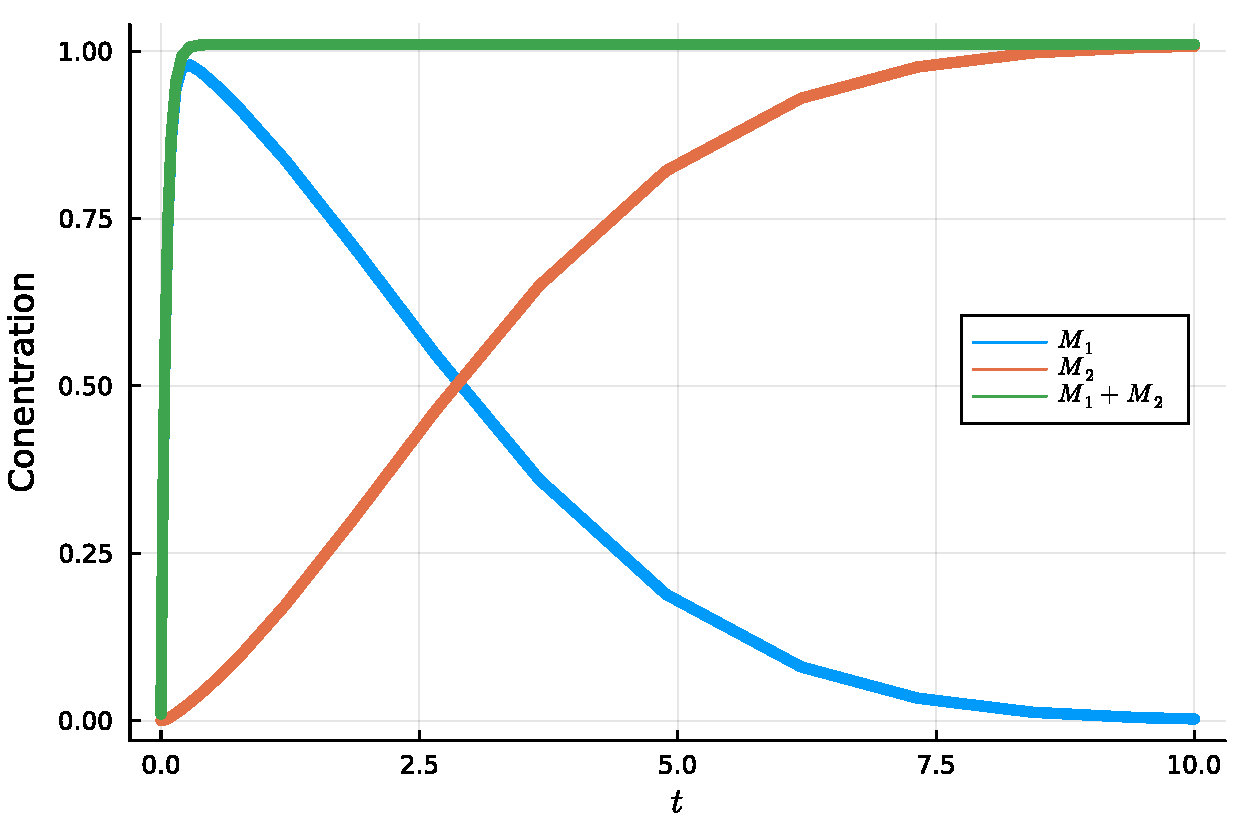
\includegraphics[width=12cm,clip]{../fig/masafig01.pdf}
        \caption{$M_1$, $M_2$, $M_1+M_2$の時系列.関数形は$f_1(t):= \gamma\exp{(-\gamma T)}$,$f_2(M_1, T_{reg}):=M_1T_{reg}$とし,パラメータは$\alpha=1.0$, $\beta=0.1$および$\gamma=20.0$とした.}
      \label{fig:01}
  \end{figure}

\end{document}